\documentclass[a4paper]{scrartcl}
\usepackage{makecell}
\usepackage{multicol}
\usepackage{graphicx}
\usepackage{anysize}
\usepackage{amsmath}
\usepackage{kpfonts}
\usepackage{tabularx}
\usepackage{hyperref}
\usepackage{listings}
\usepackage{color}

\marginsize{25mm}{25mm}{25mm}{25mm}
%---Code-Editor Config ------------------------%
\definecolor{dkgreen}{rgb}{0,0.6,0}
\definecolor{gray}{rgb}{0.5,0.5,0.5}
\definecolor{mauve}{rgb}{0.58,0,0.82}
\definecolor{backcolour}{rgb}{0.95,0.95,0.92}
\lstset{basicstyle=\ttfamily}
\lstset{literate=%
  {Ö}{{\"O}}1
  {Ä}{{\"A}}1
  {Ü}{{\"U}}1
  {ß}{{\ss}}1
  {ü}{{\"u}}1
  {ä}{{\"a}}1
  {ö}{{\"o}}1
  {é}{{\"AC}}1
  {€}{{\"AC}}1
}
\lstset{
	language=Python,				% the language of the code
	basicstyle=\footnotesize,			% the size of the fonts that are used for the code
	numbers=left,					% where to put the line-numbers
	numberstyle=\tiny\color{gray},		% the style that is used for the line-numbers
	stepnumber=1,					% the step between two line-numbers. If it's 1, each line will be numbered
	numbersep=5pt,				% how far the line-numbers are from the code
	backgroundcolor=\color{white},		% choose the background color. You must add \usepackage{color}
	showspaces=false,				% show spaces adding particular underscores
	showstringspaces=false,			% underline spaces within strings
	showtabs=false,				% show tabs within strings adding particular underscores
	frame=single,					% adds a frame around the code
	rulecolor=\color{black},			% if not set, the frame-color may be changed on line-breaks within not-black text (e.g. commens (green here))
	tabsize=2,						% sets default tabsize to 2 spaces
	captionpos=b,					% sets the caption-position to bottom
	breaklines=true,                			% sets automatic line breaking
  	breakatwhitespace=false,       		% sets if automatic breaks should only happen at whitespace
  	title=\lstname,        % show the filename of files included with \lstinputlisting; % also try caption instead of title
  	keywordstyle=\color{blue},          	% keyword style
  	commentstyle=\color{dkgreen},       	% comment style
  	stringstyle=\color{mauve},         		% string literal style
  	escapeinside={\%*}{*)},            		% if you want to add LaTeX within your code
  	morekeywords={*,...}              		% if you want to add more keywords to the set
}

%Header and Footer -----------------------%
\usepackage[headsepline]{scrlayer-scrpage}
\pagestyle{scrheadings}
\clearpairofpagestyles
%\setlength{\headheight}{40.8pt}
\setlength{\headheight}{56pt}
\ihead{IRTM\\ Wi 20/21\\ Assigment 1} 
\ohead{
    Alberto Saponaro - saponaroalberto97@gmail.com\\
    Walter Väth - walter.vaeth@gmail.com\\
    Chong Shen - st143575@stud.uni-stuttgart.de\\
    Xin Pang - st145113@stud.uni-stuttgart.de\\
}
\ofoot{\pagemark}

%-----------------------------------------------%
%  BEGIN                                        %
%-----------------------------------------------%
\begin{document}
    
\section*{Pen and Paper Task 1}
    
\subsection*{Subtask A}

\begin{itemize}
    \item sun $\rightarrow$ 1, 2, 3, 4, 7
    \item nice $\rightarrow$ 1, 5, 6
    \item water $\rightarrow$ 5, 6, 8, 9
    \item is $\rightarrow$ 6
    \item beer $\rightarrow$ 10
\end{itemize}

\subsection*{Subtask B}
\begin{figure}[ht]
    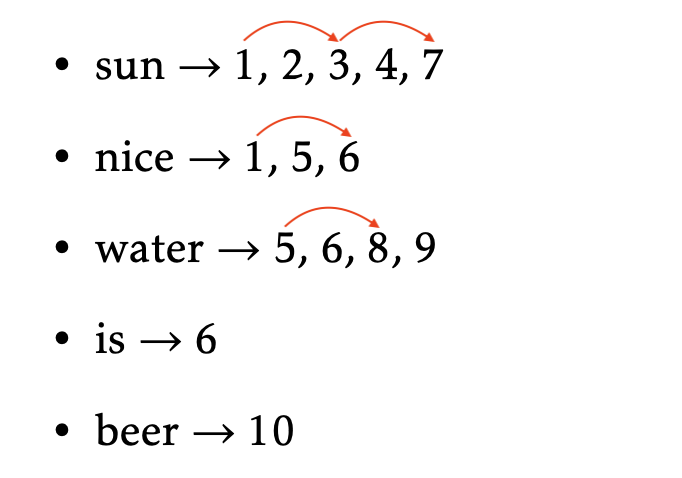
\includegraphics[width=0.4\textwidth]{img/skip_pointers.png}
\end{figure}

Example query: \textit{nice AND is}
\begin{enumerate}
  \item Comparisons without skip pointers: 1 \& 6, 5 \& 6, 6 \& 6 $\Rightarrow$ 3 comparisons
  \item Comparisons with skip pointers: 1 \& 6, 6 \& 6 $\Rightarrow$ 2 comparisons
\end{enumerate}
Without skip pointers we must compare the terms step by step, although 5 in \textbf{nice} is still smaller than 6 in \textbf{is}. With skip pointers we can skip the 5 in \textbf{nice} and directly go to the 6 in \textbf{nice}.\\

\clearpage
\section*{Pen and Paper Task 2}
\begin{figure}[ht]
    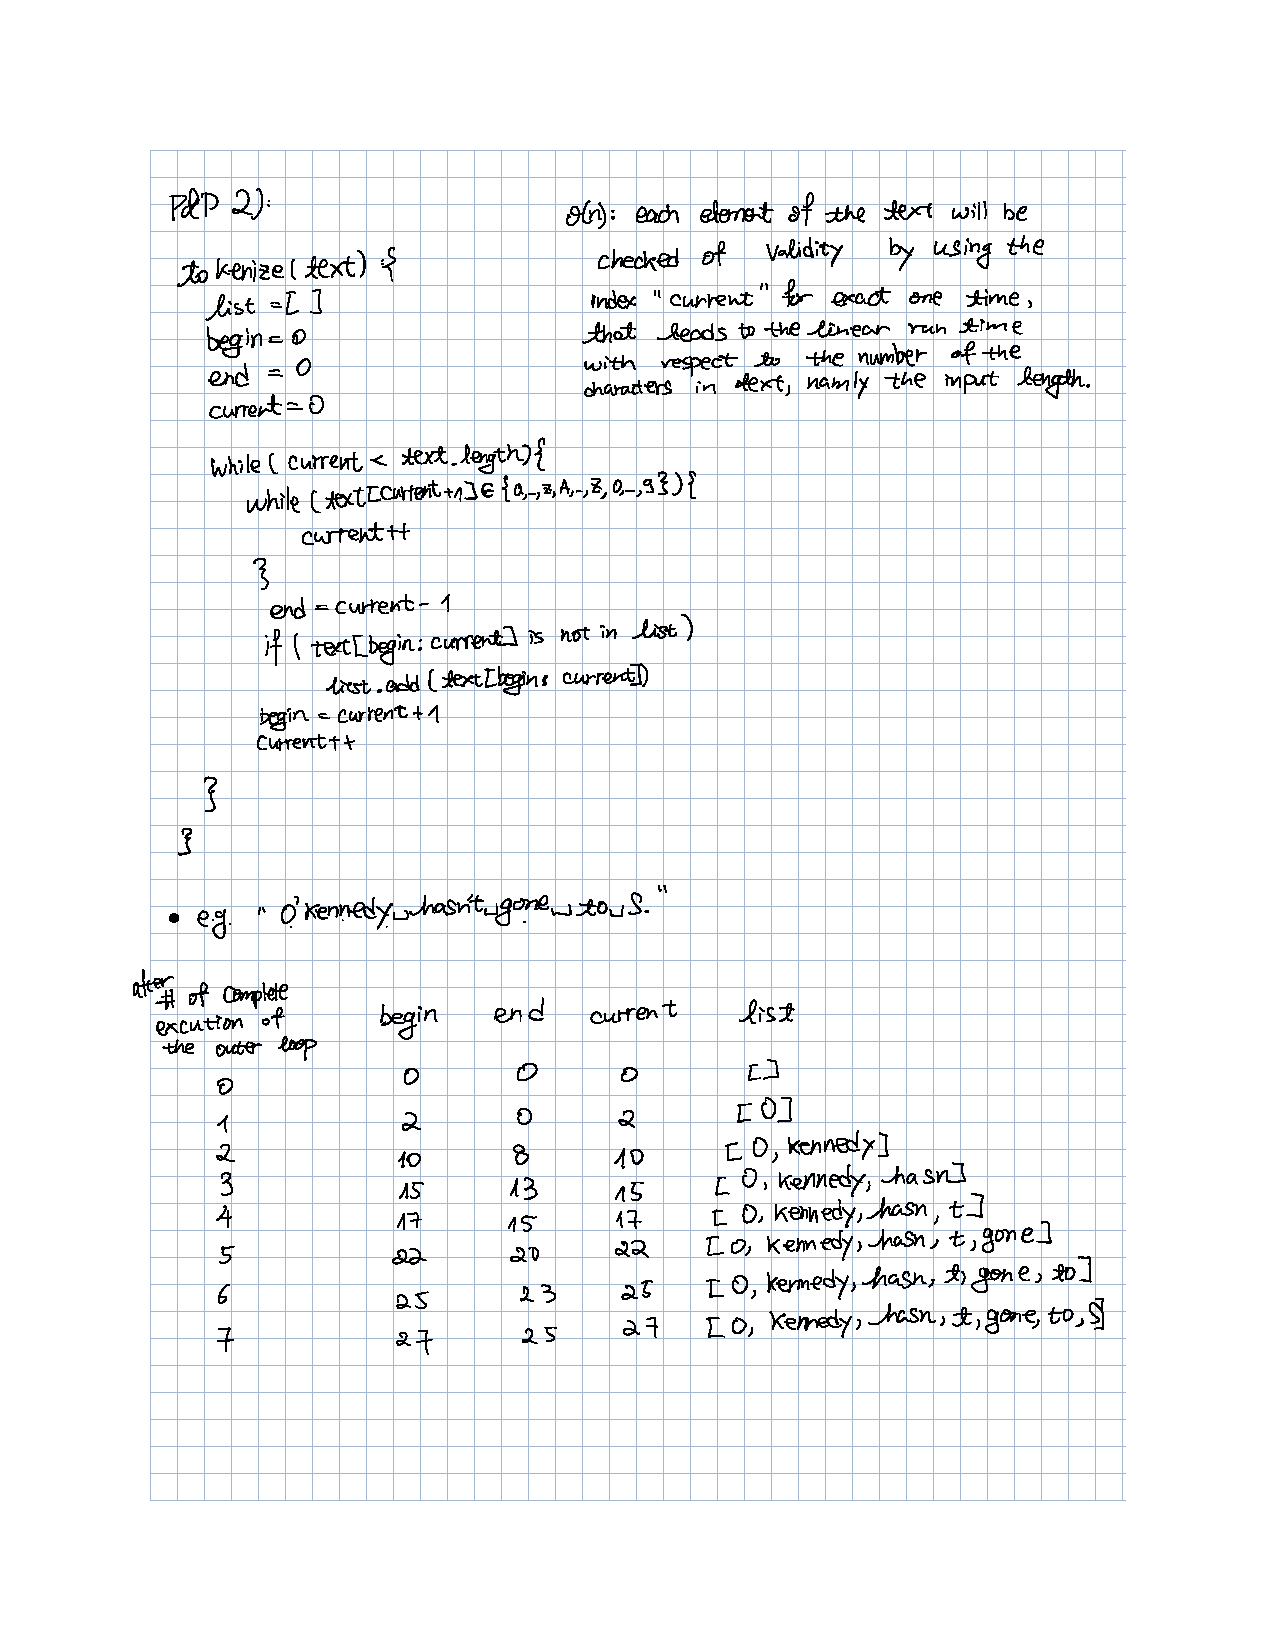
\includegraphics[width=0.8\textwidth]{img/p&p2.pdf}
\end{figure}


\clearpage
\section*{Pen and Paper Task 3}
Query: \textit{Gates /2 Microsoft}\\
\\
(Gates, 4): \quad \; [\{1:[3], 2:[6], 3:[2, 17], 4:[1]\}]\\
(Microsoft, 4): [\{1:[1], 2:[1, 21], 3:[3], 5:[16, 22, 51]\}]\\
\\
cross product = \{
  1:[(3,1)],
  2:[(6,1), (6,21)],
  3:[(2,3), (17,3)],
  4:[(1,16), (1,22), (1,51)]
\}\\
\\
From all tuples in the cross product, the tuples (3,1) and (2,3) fulfill the query's condition abs(tuple[1]-tuple[0]) $\leq$ 2. So the answer is: document 1, document 3.\\

\clearpage
\section*{Pen and Paper Task 4}
\begin{figure}[ht]
    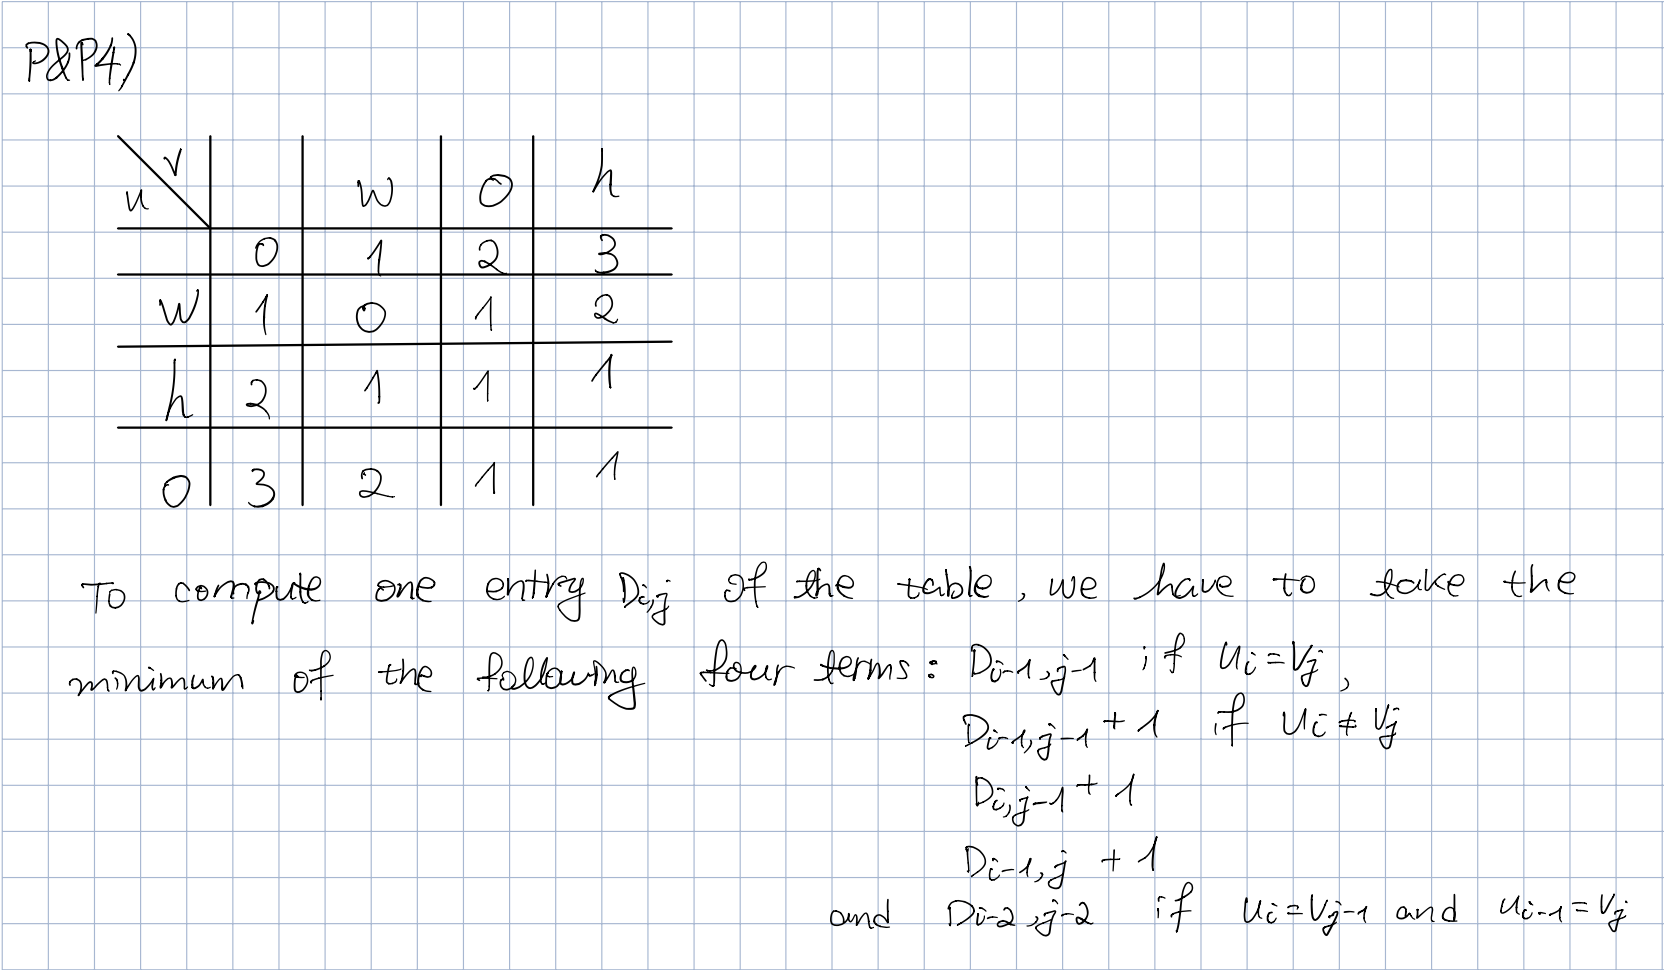
\includegraphics[width=1\textwidth]{img/p&p4.png}
\end{figure}

\clearpage
\section*{Programming Task 1}
\lstinputlisting{code/script.py}

The result shows the docID with the news text. With the use of an iterator -in Python simply a for loop- I iterate through the first and second postings list to find if the two terms are found in both documents.\\
The differences between the two queries is that in the first one we don't need an intersect algorithm.
In this case we can use the postings list of the given term directly. In the second one with two terms we have to calculate the intersection of the two postings lists and the return the text of the documents that have bouth terms in it.

\subsection*{Terminal OUTPUT:}
\begin{lstlisting}
weiß AND maß
('691', '   +++ Würde am liebsten im Erdboden versinken: Maulwurf hat das GraACben verlernt +++ +++ Aus Fluss: Schwimmerin weiß, woher sie Entzündungskrankeit hat +++ +++ Es ist ein Mädchen!: Fliege bekommt Nachwuchs +++ +++ Nur an der Nase herumgeführt: Masochist unzufrieden mit Domina-Dienstleistung +++ +++ Maß Capone: Schneider von Gangsterboss erhält Frischkäse zum Dank +++ +++ Hat Eindruck hinterlassen: Jürgen W. Möllemann +++ +++ Stehen auf der Gersteliste: Gerd Reide und Johann Hafer zu Roggen-Roll-Party eingeladen +++   Jetzt bestellen! Die besten Newsticker als Buch (nur 9,99€): Der Postillon: +++ Newsticker +++ ')

weiß AND masse
('864', '   Berlin (dpo) - Die Polizei spricht von einem gefährlichen neuen Drogen-Trend: Immer mehr Berliner begeben sich seit gestern mit Bananenresten in den Atemwegen in ärztliche Behandlung. Intensive Recherchen des Postillon im Berliner Drogenmilieu haben ergeben, dass der Ursprung der mysteriösen Fälle offenbar bei einer 140-Kilo-Lieferung eines neuen Mode-Kokains aus Kolumbien liegt, die seit Dienstagvormittag im Umlauf ist. Wie der Stoff in die Szene geraten ist, bleibt unklar.   Nach Angaben von Dealer Henrik K.* (*Name von der Redaktion geändert), der mehrere Kilogramm des neuartigen Kokains kaufte, hat die Lieferung gravierende Mängel. "Nicht einmal gerade Lines lassen sich mit dem Zeug legen", klagt der 32-Jährige.   Ist unzufrieden mit dem neuen Stoff: Henrik K.  Einige seiner Kunden, die spekulierten, dass es sich bei der neuen, gelb-gebogenen Darreichungsform um Verpackung handeln könnte und nach stundenlangem Kampf zum Inneren vordrangen, berichten von einer matschigen Masse, die zwar einigermaßen weiß, aber kein bisschen feinkörnig sei und nur die Nase verstopfe. Lediglich ein Abnehmer, der das neue Kokain im LSD-Rausch aß, habe von einem wohligen Völlegefühl berichtet und wolle unbedingt mehr von dem "Wunderzeug" kaufen. Henrik K. schöpft daraus jedoch wenig Trost: Seit gestern trocknet er 3 Kilogramm der Masse in seinem Backofen, um sie anschließend zu zermahlen und doch noch irgendwie nutzbar zu machen. "Wenn das nicht klappt, kann ich nur noch schauen, ob es vielleicht intravenös funktioniert. Sonst weiß ich auch nicht weiter." Zwar scheint eine Überdosis mit dem neuen Stoff nicht möglich, acht Konsumenten werden aber wohl bleibende Schäden davontragen. Sie leierten ihre Nasenlöcher beim Versuch, das Kokain ungeschält zu schnupfen, hoffnungslos aus.  ') 

('2197', '   Osnabrück (dpo) - Müssen Fans bald auf eine liebgewonnene Tradition verzichten? Nachdem Schiedsrichter Martin Petersen beim Pokalspiel zwischen dem VfL Osnabrück und RB Leipzig von einem Feuerzeug getroffen wurde, erwägt der DFB nun ernsthaft, das Werfen von Feuerzeugen in Fußballstadien unter Verbot zu stellen. Man befürchtet, dass von den Projektilen Verletzungsgefahr ausgeht.  "Fußball ist ein Erlebnis für die ganze Familie. Deshalb spielen wir mit dem Gedanken, Feuerzeugwürfe - so schön sie auch anzuschauen sind - zu untersagen", erklärte DFB-Präsident Wolfgang Niersbach. "Derzeit werben wir für die Zustimmung der Vereine zu dieser sicherlich umstrittenen Maßnahme."   Darf bald nur noch zum Entzünden von Pyrotechnik verwendet werden: Feuerzeug  Fan-Initiativen zeigen sich empört: "Fußball lebt von Emotionen", erklärt etwa René Finkel vom Osnabrück-Fanclub Lila-Weiß Westerkappeln. "Da gehört das Werfen von Feuerzeugen aus einer anonymen Masse einfach dazu. Was kommt als Nächstes? Ein Verbot, den Platz zu stürmen?" Tatsächlich hat der Feuerzeugwurf Tradition. Er geht zurück bis Mitte des 19. Jahrhunderts, als es üblich war, Feuersteine und Zunderdosen auf das Spielfeld zu werfen. Ziel der Würfe war es schon damals, gegnerische Spieler oder den Schiedsrichter möglichst schwer zu verletzen und einen Spielabbruch herbeizuführen. Während der Weimarer Republik geriet der Brauch nahezu in Vergessenheit. Zu wenig Wucht entwickelten die damals üblichen Streichhölzer. Erst mit der massenhaften Einführung des Feuerzeugs erlebte der Zündmittelwurf eine Renaissance. Sollte das Feuerzeugwurfverbot tatsächlich kommen, müssten zahlreiche Fanclubs und Ultra-Gruppierungen ihre Feuerzeugwurf-Bataillone auflösen oder auf andere Wurfgegenstände umlernen lassen. Auch die beliebten Wurffeuerzeug-Stände in den Stadien würden dann der Vergangenheit angehören.   ') 

('4933', '   Köln, Stuttgart, München (dpo) - Ein meteorologisches Rätsel sorgt derzeit in weiten Teilen Deutschlands für große Verunsicherung. Der Grund: In vielen Regionen fiel im Laufe des Tages eine bislang noch unbekannte nasskalte, helle Masse vom Himmel. Vielerorts blieb die Substanz liegen und färbte die Landschaft leuchtend weiß ein. Laut Behörden besteht keine Gefahr für die Bevölkerung.  "Es war unheimlich", berichtet Hausfrau Renate P. aus Stuttgart dem Postillon. "Plötzlich hab ich was Kaltes auf der Nase gespürt. Ich schau nach oben und seh, dass da so weißes Zeug runterrieselt. Ganz leise. Sah aus wie bei mir daheim in der Tiefkühltruhe." Frau P. flüchtete sich daraufhin gemeinsam mit anderen Passanten in einen Laden, wo sie mehrere Stunden lang ausharrte.    "Maaammmiiiiii! Ich hab Angst!"  Inzwischen haben Meteorologen eine Erklärung für das Phänomen parat. Demnach soll es sich nicht wie zunächst vermutet um Vulkanasche oder radioaktiven Fallout handeln. "Vielmehr haben wir es bei der weißen Substanz mit einer speziellen Form von Niederschlag zu tun, wie man sie sonst aus dem skandinavischen Raum oder aus alten Erzählungen kennt", erklärt Susanne Brauer vom Deutschen Wetterdienst. "Früher hat diese Substanz in der Winterzeit oft weite Teile Europas bedeckt." Zwar halten die Behörden den Niederschlag bislang für ungiftig, doch zumindest auf Autofahrer scheint die unbekannte Masse einen bizarren Effekt zu haben. Viele von ihnen reagieren panisch und verwirrt und scheinen innerhalb kürzester Zeit selbst die grundlegendsten Regeln des Straßenverkehrs vollständig zu vergessen. Vorerst sollen deshalb die kommunalen Winterdienste sämtliche Straßen mit extrem langsam fahrenden Räum- und Streufahrzeugen blockieren, bis sich die Lage wieder beruhigt hat.  ') 

weiss AND maße
weiss AND masse
\end{lstlisting}

\end{document}